\chapter{Électrons dans un potentiel périodique faible}
Avec un tel potentiel, on peut déjà en apprendre beaucoup car il 
va permettre d'étudier les métaux à "électrons quasi-libre", car 
on part du modèle de Sommerfeld auquel on rajoute une faible 
périodicité. Même si ce n'est pas exact, deux raisons on l'effet 
d'un potentiel faible :
\begin{enumerate}
\item Interaction ion-électron forte à petite distance mais par 
Pauli, les électrons de conductions ne peuvent rentrer dans le 
voisinage immédiat des ions à cause des électrons de cœur.
\item La mobilité des électrons dans les régions autorisées 
diminue le potentiel car ils peuvent faire écran aux ions 
chargés positivement.
\end{enumerate}

	\section{Approche générale de l'équation de Schrödinger 
	lorsque le potentiel est faible}
	On peut écrire une équation de Schrödinger modifiée 
	\begin{equation}
	H_{\vec{k}}u_{\vec{k}}(\vec{r}) = \left(\frac{\hbar^2}{2m}
	\left(\frac{1}{i}\vec{\nabla}+\vec{k}\right)^2 + U(\vec{r})
	\right)u_{\vec{k}}(\vec{r}) = \epsilon_ku_{\vec{k}}(\vec{r})
	\end{equation}
	On voit apparaître l'hamiltonien modifié, toujours un 
	opérateur hermitique impliquant que $\epsilon\in\mathbb{R}$. 
	Dès lors $H_{\vec{k}}^*u_{\vec{k}}^* = \epsilon u_{\vec{k}}^*$. 
	Comme la seule partie imaginaire est $\frac{1}{i}\vec{\nabla}$, 
	on en déduit que 
	\begin{equation}
	H_{\vec{k}}^* = H_{-\vec{k}}
	\end{equation}
	Il en découle que $\epsilon(\vec{k}) = \epsilon(-\vec{k})$, soit 
	une symétrie de translation de $\vec{k}$. Si l'on considère 
	$\vec{K} \in $ réseau réciproque, il en vient que $\epsilon(\vec{k}
	\pm\vec{K}) = \epsilon(\vec{k})$.\\
	Comme il n'y a pas de discontinuité à l'origine, $\epsilon(0)$ 
	est bien continu en cette origine.\\
	
	Avant de passer à la démonstration, commençons par un léger 
	préambule.\\
	Dans le modèle de Sommerfeld, nous considérions un potentiel 
	constant, décrit par l'équation de Schrödinger stationnaire
	\begin{equation}
	\left(-\frac{\hbar^2}{2m}\Delta + V_0\right)\psi = E\psi 
	\rightarrow \psi(\vec{r}) = \frac{1}{\sqrt{V}}e^{i\vec{k}.\vec{r}}
	\quad \ddagger\quad \frac{\hbar^2 k^2}{2m} = \epsilon-V_0
	\end{equation}
	Une solution $\ddagger$ de $\frac{1}{\sqrt{V}}e^{i(\vec{k}-\vec{k_0})
	\vec{r}}$ est également acceptable : $\frac{\hbar^2}{2m}|\vec{k}-
	\vec{k_0}|^2 = \epsilon-V_0$.\\
	On peut imposer la forme de la fonction de Bloch $\psi_{n,\vec k}(
	\vec{r}) = e^{i\vec{k}.\vec{r}}u_{n,\vec{k}}(\vec{r})$ où
	\begin{equation}
	u_{n,\vec{k}}(\vec{r}) = \sum_{\vec{K}} c_{\vec{k}-\vec{K}}e^{i\vec{K}.
	\vec{r}} \rightarrow \psi_{n,\vec{k}}(\vec{r}) = \sum_{\vec{K}} c_{\vec{k}
	-\vec{K}}e^{i(\vec{k}-\vec{K})\vec{r}}
	\end{equation}
	\danger Il faut que $\frac{\hbar^2}{2m}|\vec{k}-\vec{k_0}|$ soit 
	identique $\forall\vec{K}$ dans la combili, sans quoi ce ne serait 
	pas un état propre du même hamiltonien.\\
		\begin{wrapfigure}[10]{l}{7.5cm}
	\vspace{-0.5cm}
	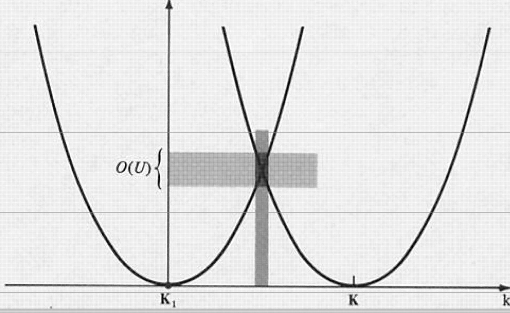
\includegraphics[scale=0.4]{ch5/image1.png}
	\captionof{figure}{ }
	\end{wrapfigure}
	Si notre réseau de Bravais a une périodicité $a$, le réseau 
	réciproque a une périodicité de $\frac{2\pi}{a}$. Considérons 
	l'énergie\footnote{Le $V_0$ disparaît dans une période??} 
	$\epsilon = \frac{\hbar^2}{2m}|\vec{k}-\vec{K}|^2$. La première 
	zone de Brilloin est ainsi définie sur $[-\frac{2\pi}{a},\frac{\pi}{
	a}]$. Les intersections se font aux limites des zones de Brilloin. A 
	ces intersections (en 2D) il existe deux combilis d'onde planes mais 
	lorsque l'on est loin des plans de Bragg (intersections) il n'existe 
	qu'une seule combili d'onde plane et on retrouve le modèle de Sommerfeld.\\
	
	Il est toujours possible de restreindre $\vec k$ à la première zone, 
	c'est-à-dire que l'on peut centrer la parabole à électron libre en tous 
	les vecteurs $\vec{K}$ du réseau réciproque\footnote{La seconde parabole 
	sur le schéma ci-dessus est équivalente à la première par translation.}. 
	Cette limitation à la première zone laisse apparaître une structure en 
	bandes.\\
	
	\textsc{Démonstration de la structure en bande}\\
	Reprenons notre potentiel périodique faible. Faible veut dire petit par 
	rapport à l'énergie cinétique des électrons. Ainsi, si $U$ varie 
	faiblement 
	\begin{equation}
	U_{\vec{K'}-\vec{K}} \ll E_C\qquad\rightsquigarrow \quad\text{Appximation 
	des électrons quasi-libres}
	\end{equation}
	Si le potentiel périodique est nul, les solutions sont des ondes 
	planes. Un bon point de départ pour les potentiels périodiques 
	faibles est le développement en solution exacte d'onde planes. Ainsi,
	reprenons l'expression apparaissant à la fin de la démonstration du 
	théorème de Bloch : 
	\begin{equation}
	\left\{\frac{\hbar^2}{2m}|\vec{k}-\vec{K}|-\varepsilon\right\}c_{
	\vec{k}-\vec{K}}+\underbrace{\sum_{\vec{K'}}U_{\vec{K'}-\vec{K}}\ 
	c_{\vec{k}-\vec{K'}	}}_{(*)}=0
	\end{equation}	
	L'approximation des électrons quasi libre implique que $(*)$ est 
	petit (et même nul dans le modèle de Sommerfeld). Nous avons ici une 
	infinité d'ondes, mais certaines ont un coefficient prépondérant.\\
	Si (approx électrons libres) les composantes de Fourier $U_{\vec{K}}$ 
	sont nuls, on peut ré-écrire l'expression comme
	\begin{equation}
	\left(\varepsilon_{\vec{k}-\vec{K}}^0 - \varepsilon\right)c_{\vec{k}
	-\vec{K}} = 0
	\end{equation}
	Cette équation implique que $c_{\vec{k}-\vec{K}}=0$ ou $\varepsilon_{\vec{k}
	-\vec{K}}^0 = \varepsilon$. Ce dernier cas se produit pour un seul $\vec{K}$ 
	sauf si $\varepsilon_{\vec{k}-\vec{K}}^0$ est égaux pour différents $\vec K$. 
	Si cette dégénérescence ne se produit pas, les solutions sont
	\begin{equation}
	\varepsilon = \varepsilon_{\vec{k}-\vec{K}}^0,\qquad \psi_{\vec{k}}(\vec{r})
	\approx e^{i(\vec{k}-\vec k)\vec{r}}
	\end{equation}
	Hélas, si $U_{\vec{K}} \neq 0$ mais petit, c'est plus subtil et il faut 
	traiter deux cas : le cas non-dégénéré et le cas dégénéré (seul le premier 
	a été vu en cours, seule le résultat du second sera exposé ici).

		\subsection{Cas 1 : quasi non-dégénérescence}
		Soit $\vec{k}$ fixé. Considérons $\vec{K_1} : \varepsilon_{\vec{k}-
		\vec{K_1}}^0 \neq \varepsilon_{\vec{k}-\vec{K}}^0\ \ \forall\vec{K}
		\neq \vec{K_1}$. On a bien évidemment
		\begin{equation}
		U \ll |\varepsilon_{\vec{k}-\vec{K_1}}^0-\varepsilon_{\vec{k}-\vec{K}}^0|
		\end{equation}
		En posant $\vec{K}=\vec{K_1}$ dans notre expression du théorème de 
		Bloch, on obtient
		\begin{equation}
		\left(\varepsilon-\varepsilon_{\vec{k}-\vec{K_1}}^0\right) = 
		\sum_{\vec{K}\neq\vec{K_1}} U_{\vec{K}-\vec{K_1}}\ c_{\vec{k}-\vec{K}}
		\end{equation}
		On utilise une constante additive afin que $U_0=0$. On peut faire 
		ressortir de la somme notre terme en $\vec{K_1}$ pour avoir un membre 
		de droite du second ordre en $U$.
		\begin{equation}
		c_{\vec{k}-\vec{K}} = \dfrac{U_{\vec{K_1}-\vec{K}}\ c_{\vec{k}-\vec{K_1}}}{
		\varepsilon-\varepsilon_{\vec{k}-\vec{K}}^0} + \sum_{\vec{K'}\neq\vec{K_1}}
		\dfrac{U_{\vec{K'}-\vec{K}}\ c_{\vec{k}-\vec{K'}}}{\epsilon - \varepsilon_{\vec{k}-
		\vec{K}}^0}
		\end{equation}
		Cette mise en évidence prend du sens car $c_{\vec{k}-\vec{K_1}}$ est d'un 
		ordre de grandeur supérieur aux autres termes\footnote{Pq ?? Et pq $U^2$?}. 
		S'il n'y a pas de dégénérescence :
		\begin{equation}
		c_{\vec{k}-\vec{K}} = \dfrac{U_{\vec{K_1}-\vec{K}}\ c_{\vec{k}-\vec{K_1}}}{
		\varepsilon-\varepsilon_{\vec{k}-\vec{K}}^0} +\mathcal{O}(U^2)
		\end{equation}
		En substituant :
		\begin{equation}
		\left(\varepsilon-\varepsilon_{\vec{k}-\vec{K_1}}^0\right)c_{\vec{k}-\vec{K_1}} = 
		\sum_{\vec{K}\neq\vec{K_1}} \dfrac{U_{\vec{K}-\vec{K_1}}\ U_{\vec{K_1}-\vec{K
		}}}{\epsilon - \varepsilon_{\vec{k}-\vec{K}}^0}c_{\vec{k}-\vec{K_1}} + 
		\mathcal{O}(U^3)
		\end{equation}
		Le niveau d'énergie perturbé\footnote{?} $\varepsilon$ diffère de 
		$\\varepsilon_{\vec{k}-	\vec{K_1}}^0$ par des termes d'ordre $U^2$. On remplace 
		ainsi $\varepsilon$ par $\epsilon - \varepsilon_{\vec{k}-
		\vec{K_1}}^0$ pour avoir
		\begin{equation}
		\varepsilon =  \varepsilon_{\vec{k}-	\vec{K_1}}^0+ \sum_{\vec{K'}} 
		\dfrac{|U_{\vec{K}-\vec{K_1}}|^2}{\varepsilon_{\vec{k}-\vec{K_1}}^0 - 
		\varepsilon_{\vec{k}-\vec{K}}^0} + \mathcal{O}(U^3)
		\end{equation}
		Cette expression exprime que les bandes non-dégénérées se repoussent. Ce 
		qu'il faut retenir est que dans le cas de quasi non-dégénérescence l'énergie 
		est décallée par rapport à l'énergie d'électrons libre de termes en $|U|^2$.
		
		
		\subsection{Cas 2 : quasi dégénérescence}
		En faisant des calculs similaires, on peut déterminer à une précision de 
		l'ordre de $U^2$ les décalages des $m$ niveaux quasi-dégénérés en résolvant 
		$m$ équations. Cette expression peut être simplifiée en 
		\begin{equation}
		\left(\varepsilon-\varepsilon_{\vec{k}-\vec{K_i}}^0\right)c_{\vec{k}-\vec{K_i}} =
		\sum_{j=1}^m U_{\vec{K_j}-\vec{K_u}}\ c_{\vec{k}-\vec{K_j}}
		\label{eq:quasiD}
		\end{equation}
		
	\section{Niveaux d'énergie près d'un plan de Bragg unique}
	Considérons deux niveaux distincts de l'ordre de $U$ l'un de l'autre, mais très 
	différent des autres : on a donc un cas de quasi-dégénérescence et \autoref{eq:quasiD} 
	se déduit à 
	\begin{equation}
	\begin{array}{ll}
	\left(\varepsilon-\varepsilon_{\vec{k}-\vec{K_1}}^0\right)c_{\vec{k}-\vec{K_1}} &=
	U_{\vec{K_2}-\vec{K_1}}\ c_{\vec{k}-\vec{K_2}}\\
	\left(\varepsilon-\varepsilon_{\vec{k}-\vec{K_2}}^0\right)c_{\vec{k}-\vec{K_2}} &=
	U_{\vec{K_1}-\vec{K_2}}\ c_{\vec{k}-\vec{K_1}}	
	\end{array}
	\end{equation}
	Comme il n'y a que deux niveaux, introduisons des notations plus simples :
	$\vec{q} = \vec{k}-\vec{K_1}$ et $\vec{K}=\vec{K_2}-\vec{K_1}$ pour avoir :
	\begin{equation}
	\begin{array}{ll}
	\left(\varepsilon-\varepsilon_{\vec{q}}^0\right)c_{\vec{q}} &= U_{\vec{K}}\ c_{
	\vec{q}-\vec{K}}\\
	\left(\varepsilon-\varepsilon_{\vec{q}-\vec{K}}^0\right)c_{\vec{q}-\vec{K}} &= 
	U_{-\vec{K}}\ c_{\vec{q}} = U_{+\vec{K}}^*\ c_{\vec{q}}
	\end{array}	
	\end{equation}
	On a $\varepsilon_{\vec{q}}^0=\varepsilon_{\vec{q}-\vec{K}}^0 \Leftrightarrow |
	\vec{q}|=|\vec{q}-\vec{K}|$ impliquant que $\vec{q}$ soit se trouver sur le plan 
	de Bragg. Cela signifie donc que $\vec{k}$ est proche du plan de Bragg mais pas 
	d'un point ou cex plans se coupent. LE cas de deux niveaux générés s'applique à 
	un électron dont le vecteur d'onde $\vec{k}$ satisfait approximativement la 
	condition pour une diffraction de Bragg unique.\\
	
	Les niveaux quasi-dégénérés sont les plus affecté par un potentiel périodique. 
	Ce potentiel à ses effets principaux sur les niveaux d'électrons libres dont les 
	vecteurs d'onde sont proche de ceux pour lesquels les réflexion de Bragg peuvent 
	se produire. Examinons la structure des niveaux avec une diffraction de Bragg 
	unique :
	\begin{equation}
	\left|\begin{array}{cc}
	\varepsilon-\varepsilon_{\vec{q}}^0 & -U_{\vec{K}}\\
	-U_{\vec{K}}^* & \varepsilon - \varepsilon_{\vec{q}-\vec{K}}^0
	\end{array}\right| = 0
	\end{equation}
	Les deux solutions de cette équations sont \\
	\begin{wrapfigure}[10]{r}{3.5cm}
	\vspace{-1.5cm}
	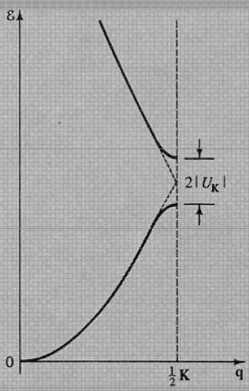
\includegraphics[scale=0.4]{ch5/image2.png}
	\captionof{figure}{ }
	\end{wrapfigure}
	\vspace{-1cm}
	\begin{equation}
	\varepsilon = \frac{1}{2}\left(\varepsilon_{\vec{q}}^0+\varepsilon_{\vec{q}-
	\vec{K}}^0\right) \pm \left[\left(\dfrac{\varepsilon_{\vec{q}}^0 - \varepsilon_{
	 \vec{q}-\vec{K}}^0}{2}\right)^2 + |U_{\vec{K}}|^2\right]^{1/2}
	\end{equation}
	Sur les plans de Bragg, on a une égalité entre les $\varepsilon$ donnant lieu à
	\begin{equation}
	\varepsilon = \varepsilon_{\vec{q}}^0 \pm |U_{\vec{K}}|
	\end{equation}
	sur le plan de Bragg simple. En tout point sur le plan de Bragg, un niveau est 
	augmenté de $|U_{\vec{K}}|$ et l'autre diminué de $|U_{\vec{K}}|$ : ceci provoque 
	une levée de la dégénérescence et un gap de $2|U_{\vec{K}}|$.
	
	\section{Bandes d'énergies à une dimension}
	Seule les doubles dégénérescences peuvent se produire. Sans interactions, les 
	niveaux sont paraboliques. Avec, c'est presque pareil sauf près des plans de 
	Bragg (point en 1D) où on lève la dégénérescence de $2|U_{\vec{K}}|$. La courbe 
	originale est modifiée de façon à inclure ces coefficients de Fourier et cette 
	représentation (e) est le \textit{schéma en zone étendue}. Si l'on les représente 
	tous dans la première zone de Brillouin (e) on a le \textit{schéma en zone 
	réduite.} On peut également insister sur la périodicité (g) avec le \textit{schéma 
	en zone répétée}.
	
	\section{Courbes énergies : $\vec{k}$ en 3D}
	Plus informatif, lire la page 115.
	
	\section{Le gap en énergie}\ 
	\begin{wrapfigure}[36]{l}{11.1cm}
	\vspace{-1.4cm}
	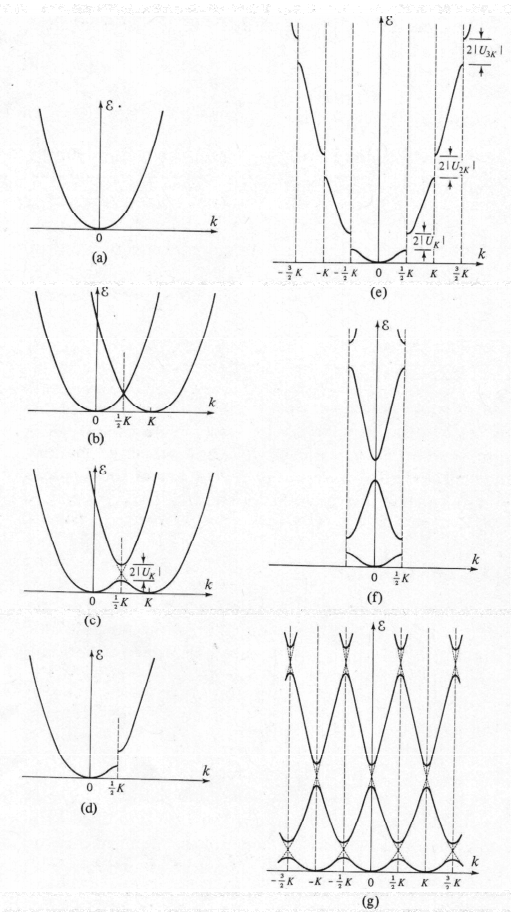
\includegraphics[scale=0.6]{ch5/image3.png}
	\captionof{figure}{ }
	\end{wrapfigure}
	Le potentiel faible introduit un gap en énergie aux plan de Bragg : l'énergie 
	varie de façon discontinue d'au moins $2|U_{\vec{K}}|$.\\
		
	En (a), nous avons une parabole en $k=0$. En (b), deux paraboles qui n'ont qu'une 
	seule interesection. En (c), si on considère en ce point la levée de la dégénérescence 
	du au potentiel périodique faible, les deux courbes se séparent et une forme de 
	structure en bande apparaît. Si on applique ceci en tous les points (e), on voit de 
	façon claire la structure en bande, c'est le schéma en zone étendue (chaque parabole 
	est dans une zone de Brillouin différente). On peut translater chacune parabole de 
	$\vec{K}$ pour obtenir (f), le schéma en zone restreinte (car $\vec k$ est restreint 
	à la première zone). Ces deux schémas sont équivalent. On peut répéter cette structure 
	dans chaque zone (g), mais on représentera alors plusieurs fois le même état physique. 
	
	
	\newpage
	\begin{wrapfigure}[12]{r}{6.5cm}
%	\vspace{-1.5cm}
	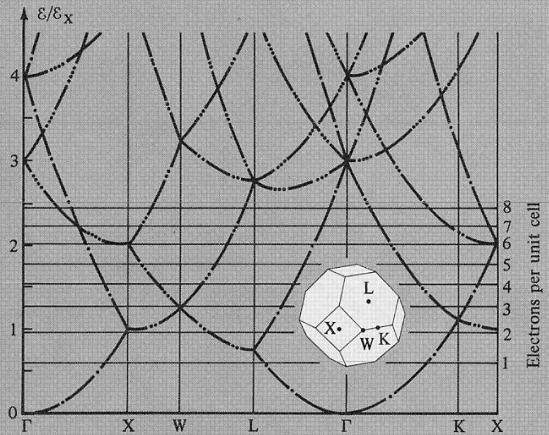
\includegraphics[scale=0.4]{ch5/image4.png}
	\captionof{figure}{ }
	\end{wrapfigure}
	
	Il existe d'autres représentation des niveaux d'énergies du modèle de Sommerfeld. Le 
	schéma suivant est obtenu en suivant des lignes de symétrie à l'intérieur des zones 
	de Brillouin. $\Gamma$ est le centre de la première zone de Brillouin. Entre $\Gamma$ 
	et $L$, on a suivi une direction de symétrie (on a été de $\Gamma$ vers le centre d'une 
	zone hexagonale, qui est un point $L$. \\
	Les bandes d'énergies représentées sont celles d'une énergie $\frac{\hbar^2}{2m}|\vec k
	-\vec K|^2$. On suit ainsi un chemin $XWKL$ pour représenter ces bandes d'énergies : 
	il s'agit du modèle de Sommerfeld, ce qui se passe quand on considère un potentiel faible 
	mais non constant.	Notons que la zone de Fermi se voit modifié aux plans de Bragg.
	
	\section{Zone de Brillouin}
	Pour les électrons libres centrés en $\vec{k}=\vec 0$, la surface de Fermi 
	est une sphère. Cette sphère va se déformer d'une certaine sorte lorsqu'elle 
	traverse un plan de Bragg (et ainsi de suite). En prenant tous les plans de 
	Bragg en compte, on retrouve une sphère fracturée dans un schéma en zone 
	étendue (répéter le schéma ci-dessous). On peut généraliser cette procédure 
	grâce aux zones de Brillouin.
	
	\begin{center}
	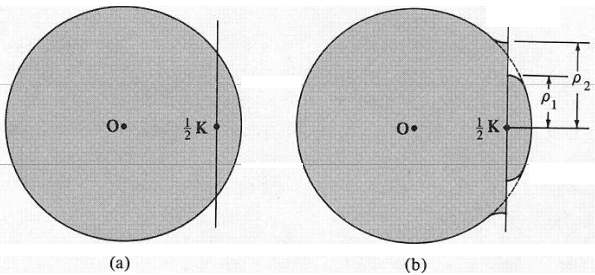
\includegraphics[scale=0.46]{ch5/image5.png}
	\captionof{figure}{Déformation de la sphère de Fermi aux plans de Bragg}	
	\end{center}

	\begin{wrapfigure}[15]{l}{7.5cm}
	\vspace{-0.5cm}
	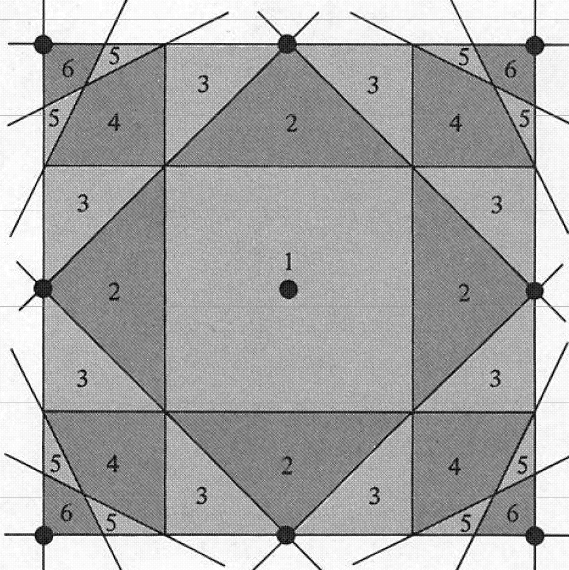
\includegraphics[scale=0.34]{ch5/image6.png}
	\captionof{figure}{Zone de Brillouin pour un réseau $2D$ carré}
	\end{wrapfigure}	
	La première zone de Brillouin est la cellule primitive de Wigner-Seitz du 
	réseau réciproque, c'est-à-dire l'ensemble des points se trouvant plus 
	proche de $\vec{K}=\vec{0}$ que de n'importe quel autre vecteur  du réseau 
	réciproque. Or les plans de Bragg sont les plans médiateurs des lignes 
	joignant l'origine à des points du réseau réciproque. On peut donc définir 
	la première zone de Brillouin comme l'ensemble des points pouvant être 
	atteints à partir de la première zone sans traverser un seul plan de Bragg. 
	La seconde zone de Brillouin si on a traversé un plan de Bragg, \dots\\
	
	La $n^e$ zone de Brillouin est l'ensemble des points qui peuvent être 
	atteints à partir de l'origine en traversant $(n-1)$ plans de Bragg 
	(sans retour arrière). L'interprétation physique de ceci est que les 
	zones sont bornées par les plans de Bragg. Il existe un algorithme 
	pour construire les branches de la surface de Fermi :
	\begin{enumerate}
	\item Dessiner la sphère à électron libre
	\item La déformer légèrement dans le voisinage du plan de Bragg
	\item Prendre la portion de la sphère de la $n^e$ zone et la translater 
	pour tout vecteur du réseau réciproque
	\end{enumerate}
	
	\begin{center}
	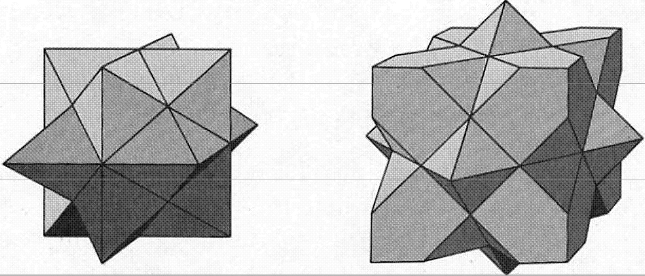
\includegraphics[scale=0.46]{ch5/image7.png}
	\captionof{figure}{Surface limitant la $2^e$ zone de Brillouin pour un 
	réseau $cc$ et $cfc$}
	\end{center}

	\begin{wrapfigure}[9]{l}{3.5cm}
	\vspace{-0.5cm}
	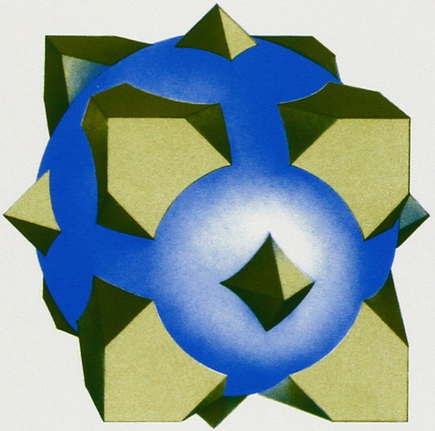
\includegraphics[scale=0.2]{ch5/image8.png}
	\captionof{figure}{ }
	\end{wrapfigure}		
	Il peut également être intéressant de superposer la surface qui délimite 
	la seconde zone de Brillouin avec la sphère de Fermi. Rappellons que chaque 
	zone comporte $2n$ états possibles (spin).\\
	Le volume de la \textbf{première} zone de Brillouin correspond à la moitié du 
	volume de la sphère de Fermi en $3D$ : tous les états dans cette première zone, 
	cette première bande, sont totalement occupé. \\
	Par contre, le volume de la \textbf{seconde} zone de Brillouin est supérieur 
	au volume de la sphère de Fermi. Des "bouts de surfaces" dépassent la sphère : 
	ce sont des niveaux inoccupés ($(a)$). Si on translate ces morceaux (qui sont 
	en réalité dans la seconde zone de Brillouin) dans la première zone, on obtient 
	le schéma $(c)$ (schéma en zone restreinte).\\

	\begin{wrapfigure}[15]{r}{7.5cm}
	\vspace{-1.3cm}
	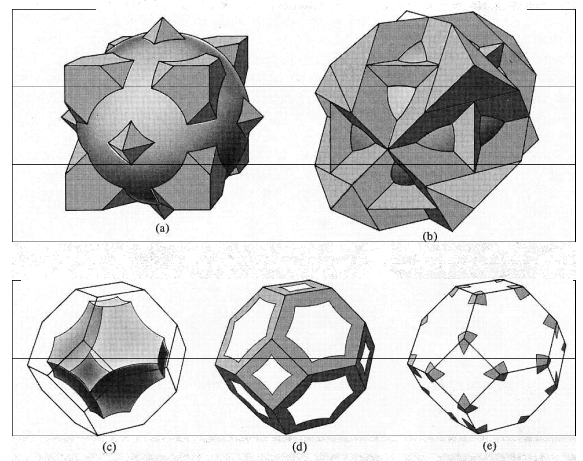
\includegraphics[scale=0.5]{ch5/image9.png}
	\captionof{figure}{ }
	\end{wrapfigure}		
	Le schéma $(b)$ est la surface délimitant la troisième zone de Brillouin. Les 
	bouts dépassant la sphère sont dans la quatrième zone. \\
	
	De façon générale, l'effet du potentiel périodique est d'"arrondir les bords".

\ \\


	\danger Les sections 8.7 et 8.8 n'ont pas été vues\\
	 au cours (no stress, au pire 
	ce ne sont que deux\\ pages).








































	